\documentclass[11pt, fleqn]{article}
\usepackage{multicol}

%\usepackage[a4, frame, center, noinfo]{crop}

%بسم الله الرحمن الرحیم

%You should edit DSLecture.tex, not this file!
\usepackage{amsthm}
\usepackage{latexsym}
\usepackage{amssymb}
\usepackage{verbatim}
\usepackage{enumitem,amsmath,array}
\usepackage{tikz}
\usepackage{tkz-graph}
\usepackage{bookmark}
\usetikzlibrary{positioning,chains,fit,shapes,calc}
%a4paper, margin=0.7in     , paperwidth=16cm,paperheight=24cm
%\usepackage[paperwidth=20cm,paperheight=29cm]{geometry}
\usepackage[a4paper, margin=0.7in]{geometry}
\usepackage{listings}
\usepackage{clrscode3e}
\usepackage{hyperref}
\hypersetup{
	colorlinks=true,
	linkcolor=blue,
	filecolor=magenta,      
	urlcolor=cyan,
}
\usepackage{xepersian}
%\usepackage[fontsloadable]{xepersian}

\settextfont{HM XNiloofar}
%\setdigitfont{HM XNiloofar}
%\setdigitfont{ParsiDigits}
\defpersianfont\outline[Scale=1]{HM XNiloofar Outline}

\setlength{\parindent}{1.5em}
\setlength{\parskip}{0.9em}
\renewcommand{\baselinestretch}{1.4}


\newcommand{\lecture}[3]{
%\pagestyle{empty}
{
	\begin{center}
			\vspace{-1cm}
		   
\includegraphics[scale=0.35]{Sharif}%\hfill \\[1em]  
	\end{center}
	\vspace{-8mm}

%\bf

%\begin{outline} 

%\end{outline} 

}\vspace*{-1em}
\noindent
 #2 \hfill 
\vspace{-4mm}
\rule{\textwidth}{1pt}
\ \\
}

% example environment
\newenvironment{example}
{\smallskip \noindent \emph{مثال:}}
{\hfill $\boxtimes$ \smallskip}


\newtheorem{theorem}{قضیه}
\newtheorem{proposition}{گزاره}
\newtheorem{claim}{ادعا}
\newtheorem{lemma}{لم}
\newtheorem{corollary}{نتیجه}
\newtheorem{definition}{تعریف} % Use this for non-trivial definitions.
\newcommand*{\newtitle}[1]{
\begin{large}
\textbf{#1}
\end{large}
}
\newcommand*{\newhline}{
\vspace{-7mm}
\rule{\textwidth}{1pt}

}
\newcommand*{\newsline}{
\vspace{-7mm}
\rule{8cm}{1pt}

}
\newcommand*{\maintitle}[1]{
\begin{center}
\textbf{
\LARGE{#1}
}
\end{center}
}
 %%%%%%%%%%%%%%%%%%%%%%%%%%%%%%%%%%%%%%%%%%%%%%%%%%%%%%%%%%%%%%%%%%%%%%%%%%%%


\usepackage{mathtools, nccmath}
\usepackage{tikz}
\usepackage{mathtools}
\usepackage{graphicx}
\usepackage{tikz} % To generate the plot from csv
\usepackage{pgfplots}
\pgfplotsset{compat=1.5}
\usetikzlibrary{patterns}
\usepackage{amssymb}% http://ctan.org/pkg/amssymb
\usepackage{pifont}% http://ctan.org/pkg/pifont
\usepackage{graphicx}

\usepackage{pgf}
\usepackage{pgfpages}

%\pgfpagesdeclarelayout{boxed}
%{
%  \edef\pgfpageoptionborder{0pt}
%}
%{
%  \pgfpagesphysicalpageoptions
%  {%
%    logical pages=1,%
%  }
%
%  \pgfpageslogicalpageoptions{1}
%  {
%    border code=\pgfsetlinewidth{2pt}\pgfstroke,%
%    border shrink=\pgfpageoptionborder,%
%    resized width=.95\pgfphysicalwidth,%
%    resized height=.95\pgfphysicalheight,%
%    center=\pgfpoint{.5\pgfphysicalwidth}{.5\pgfphysicalheight}%
%  }%
%}
%\pgfpagesuselayout{boxed}




%\usepackage{tikz}
%\usepackage{tikzpagenodes}
%\usetikzlibrary{calc}
%\usepackage{fancyhdr}

%\newcommand{\myborder}{
%\tikz[overlay,remember picture]\draw($(current page.north east)+(-1.5cm,-1.5cm)$)--($(current page.north west)+(1.5cm,-1.5cm)$)--($(current page.south west)+(1.5cm,1.5cm)$)--($(current page.south east)+(-1.5cm,1.5cm)$)--cycle;}

%\pagestyle{fancy}
%\fancyhf{}
%\renewcommand{\headrulewidth}{0pt}
%\rhead{\myborder}













\begin{document}

\renewcommand\refname{}


%\lecture{1}{}{}



\begin{center}

			\vspace{-1cm}
		   
\includegraphics[scale=0.35]{Sharif}%\hfill \\[1em]  
		   \vspace{2cm}

\textbf{
\Huge{
تخمینی از مدل رشد اقتصادی سولو-کاب-داگلاس
\LTRfootnote{Solow-Cobb-Douglas}
با استفاده از فیلتر‌های کالمن
\LTRfootnote{Kalman}
: روشی بر مبنای مشاهده پذیری
}}
\vspace{2cm}

\textbf{
\huge{
اقتصاد کلان دوره‌ی فرعی
}}
\vspace{1mm}

\textbf{
\huge{
جناب آقای دکتر بخشی‌آنی
}}

\vspace{10mm}

\textbf{
\Large{
گروه اول
\\}}
\Large{

ارشیا اکبری
\\
فاطمه توحیدیان
\\
امین کشیری
\\
ساحل مس فروش
}

\vspace{3cm}

\large{
بهار ۱۴۰۰
}
\end{center}


\newpage
\newtitle{چکیده}






\newhline

در این مقاله از یک رویکرد جدید برای تخمین مدل رشد اقتصادی سولو-کاب-داگلاس استفاده شده است. برای تخمین‌زدن پارامتر‌های متغیر خود سیستم و حالات داخلی سیستم، از یک فیلتر کالمان توسعه‌یافته 
\LTRfootnote{Extended Kalman Filter}
 یا
 EKF
 استفاده شده است. بر خلاف تکنیک‌های سنتی، در این روش تمامی پارامتر‌ها متغیر (در زمان) در نظر گرفته می‌شوند. در نهایت توانستیم همروندی خوبی در برخی از متغیر‌ها به دست آوریم و تا حدی روند رشد متغیرها را در آینده پیش بینی کنیم. روند تغییر پارامتر‌های کلان برای ایران خطی نیست، اما به دلیل این که مدل ما تغییرات پارامتر‌ها را خطی در نظر می‌گیرد،توانسته است روند تغییرات را پیش‌بینی کند.
 
 
\newhline




























\begin{multicols}{2}

\newtitle{۱. مقدمه}


	یکی از مدل‌های مهم رشد درون‌زا مدل سولو-سوان
\LTRfootnote{Solow-swan}
 است. این مدل دینامیک بلندمدت رشد اقتصادی را بر اساس انباشت سرمایه، نیروی کار و جمعیت و افزایش بهره‌وری (همان سطح تکنولوژی) توضیح می‌دهد. 
 
 
 
 
 تخمین پارامتر‌ها در توضیح دقیق رفتار سیستم مدل‌های دینامیکی مثل مدل سولو-سوان نقشی حیاتی بازی می‌کند. در مقاله‌ی
 \cite{main}
یکی از روش‌های این تخمین با استفاده از فیلتر‌هایی مثل فیلتر کالمان
\LTRfootnote{Kalman Filter}
نشان داده شده است.  


فیلتر کالمان الگوریتمی است که توسط رودولف کالمان 
\LTRfootnote{Rudolf E. Kalam}
توسعه داده شد، که از آن‌ برای تخمین حالات یک سیستم‌ دینامیکی با استفاده از اندازه‌‌گیری‌هایی در طول زمان استفاده می‌شود.

 خانواده‌‌های دیگری از الگوریتم‌ها برای حل مسائل فیلتر کردن و تخمین زدن نیز وجود دارند. نمونه‌هایی از این روش‌ها، روش‌های فیلتر‌ ذره‌ای 
\LTRfootnote{Particle Filters}
 یا روش‌های توسعه‌ یافته‌تری از فیلتر کالمان مانند فیلتر کالمان توسعه یافته 
 \LTRfootnote{Extended Kalman filter}
 (
 EKF
 ) و یا فیلتر کالمان بدون رایحه
\LTRfootnote{Unscented Kalman filter} 
(
UKF
)
هستند.
 
 
 
در مقاله‌ی
\cite{main}
، از یک فیلتر کالمان توسعه‌یافته یا
 EKF
  برای تخمین حالت یک مدل رشد اقتصادی سولو-کاب-داگلاس استفاده شده است. به این دلیل از این روش استفاده شده است که بتوانیم به صورت همزمان پارامتر‌های خود مدل و حالات داخلی سیستم را همزمان تخمین بزنیم.
دقت کنید که بر خلاف روش‌های سنتی مثل رگرسیون خطی، که پارامتر‌های سیستم ثابت فرض می‌شوند، در نمایش ارائه داده شده تمام پارامتر‌های مدل به عنوان متغیر حالت در نظر گرفته شده‌اند. 

در مقاله‌ی
\cite{main}
با استفاده از  یک آنالیز گسترده‌ی مشاهده‌پذیری، مشاهده‌پذیری مدل سولو-کاب-داگلاس بررسی شده است. با استفاده از این آنالیز، شرایط ضروری برای مشاهده‌پذیر بودن به دست آمده‌اند. این شرایط برای تخمین حالت کل سیستم با استفاده از زیرمجموعه‌ای از اندازه‌ها نیاز هستند. در نهایت با استفاده از EKF و داده‌های واقعی، این نتایج صحت‌سنجی شده‌اند. 

































\newtitle{۲. مدل}

	مدل استفاده شده در مقاله‌ی ما مدل اقتصادی سولو است که مراحل به دست آوردن آن را می‌توانید در مقاله‌ی
\cite{main}
به صورت کامل مشاهده کنید. در این مدل، فرض‌هایی وجود دارند که به صورت خلاصه آن‌ها را بیان می‌کنیم:

\begin{itemize}
\item
فرض می‌کنیم تمام سرمایه‌گذاری روی سرمایه‌ی فیزیکی مصرف می‌شود. در این صورت تغییرات سرمایه‌‌ی فیزیکی برابر است با کل سرمایه‌گذاری منهای میزان سرمایه از دست رفته به دلیل استهلاک.

\item
تمام پس‌انداز مردم روی سرمایه‌ی فیزیکی سرمایه‌گذاری می‌شود. 

\item
 فرض می‌کنیم که تولید به دو عامل نیروی‌ کار L و سرمایه‌ی کل K بستگی دارد. 

\item
 فرض می‌کنیم که تابع تولید خاصیت برگشت به مقیاس ثابت
\LTRfootnote{Constant return to scale}
	 دارد یعنی:

\begin{latin}
$F(\lambda L, \lambda K) = \lambda F(L, K)$
\end{latin}

\end{itemize}



	یکی از توابع تولیدی که شرایط تابع تولید سولو را ارضا می‌کند تابع کاب-داگلاس است:

\useshortskip
\begin{LTR}
\begin{equation}
F(K, L) = AL^\alpha K^{(1-\alpha)}
\end{equation}
\end{LTR}

که در اینجا A ضریب بهره‌وری
\LTRfootnote{Total Productivity Factor}
 (سطح تکنولوژی) و 
 $\alpha$
  کشش نیروی‌ کار است.
  
  
با استفاده از مدل سولو و تابع تولید کاب داگلاس، در نهایت به رابطه‌ی زیر برای تغییرات سرمایه به ازای هر فرد می‌رسیم:


\useshortskip
\begin{LTR}
\begin{equation}
\dot{k} = s A K^{(1-\alpha)} - (\delta + n)k
\end{equation}
\end{LTR}

که در آن
$n = \frac{\dot{L}}{L}$
نرخ رشد جمعیت،
$k = \frac{K}{L}$
 سرمایه به ازای هر فرد،
 $\delta$
  نرخ استهلاک سرمایه موجود و 
$f(k) = F(\frac{K}{L}, 1)$
. معمولا فرض می‌شود که 
 $f(k)$
 یک تابع صعودی و اکیدا مقعر است. 



	




	برای این که روی داده‌های واقعی مدل کاب-داگلاس را اعمال کنیم، مقادیر 
$\alpha$
	و A را نیاز داریم. در روش‌های سنتی مثل رگرسیون خطی این پارامترها با کمک داده‌های
Y
،
K
 و L به دست می‌آیند. در تمام روش‌های سنتی، A و 
 $\alpha$
  ثابت تخمین زده می‌شوند در صورتی که واقعا متغیرند. ما در این مقاله، تمامی پارامتر‌ها را متغیر در نظر می‌گیریم، و فرض می‌کنیم که نرخ تغییرات هرکدام از آن‌ها ثابت است. 

	با در نظر گرفتن تمامی فرض‌های بالا، نمایش حالت-فضا برای مدل ما به صورت زیر می‌شود:

\useshortskip
\begin{LTR}
\begin{equation}
\label{3}
\begin{cases}
\dot{k} = sAk^{(1-\alpha)} - (\delta + n)k

\\

\dot{A} = v_A & \dot{v_A} = 0  

\\

\dot{a} = v_a & \dot{v_a} = 0  

\\

\dot{s} = v_s & \dot{v_s} = 0  

\\

\dot{\delta} = v_\delta & \dot{v_\delta} = 0  

\\

\dot{n} = v_n & \dot{v_n} = 0  

\end{cases}
\end{equation}
\end{LTR}


که 
$v_i$
 نشان دهنده‌ی سرعت تغییرات متغیر $i$
 است. در این فضا سرعت تغییرات ثابت در نظر گرفته شده است که بتوانیم در عین سادگی، تغییرات آن‌ها با زمان را نیز در نظر بگیریم. 






























\newtitle{۳. آنالیز}

	یک سیستم را مشاهده‌پذیر می‌گوییم اگر برای هر زمانی مثل 
$t_0$
،
	 با داشتن مدل تغییر حالت
\LTRfootnote{State transition model}
(تابع 
$\mathbf{f}$
)
:

\begin{latin}
$\mathbf{\dot{x}} = \mathbf{f}(\mathbf{x})$
\end{latin}

 مدل مشاهده
\LTRfootnote{Observation model}
(تابع 
$h$
)
:

\begin{latin}
$\mathbf{y} = h(\mathbf{x})$
\end{latin}

و مشاهدات در بازه‌ی 
$t_0$
 تا 
 $t$
  یعنی
$\mathbf{z}[t_0, t]$
 بتوانیم حالت اولیه یا 
 $x_0$
 را به دست آوریم. در واقع اگر سیستمی مشاهده‌ پذیر باشد، ما می‌توانیم در مدت زمانی متناهی با اندازه گیری خروجی‌های سیستم، تمام حالات درونی‌اش را تخمین بزنیم.  
 
	در مقاله‌ی ما، بردار حالت به صورت زیر است:

\useshortskip
\begin{LTR}
\begin{equation}
\mathbf{x} = [\ k \ A \ v_A \  \alpha \  v_\alpha \  s \ v_s  \ \delta \  v_\delta \ n \  v_n \ ]^T
\end{equation} 
\end{LTR}

همچنین فرض می‌کنیم که اندازه‌های زیر از داده‌های اقتصاد کلان وجود دارند:

\useshortskip
\begin{LTR}
\begin{equation}
\mathbf{z} = [\ k \ s \ \delta \ n \ Y_L \ ]^T
\end{equation}
\end{LTR}


که در آن 
 $Y_L = \frac{Y}{L}$
  . 

	هر کدام از اندازه‌های بردار z از بردار حالت به دست می‌آید، و در واقع مدل مشاهده به صورت زیر است:

\useshortskip
\begin{LTR}
\begin{equation}
\begin{cases}
h_1(\mathbf{x}) = k \\
 h_2(\mathbf{x}) = s \\
  h_3(\mathbf{x}) = \delta \\
   h_4(\mathbf{x}) = n \\
    h_5(\mathbf{x}) = AK^{(1-\alpha)} \end{cases}
\end{equation}
\end{LTR}


	در مقاله‌ی هرمان و کرنر 
\LTRfootnote{Herman and Krener}
نشان‌داده شده است که یک سیستم غیرخطی به صورت ضعیف و محلی مشاهده‌پذیر
\LTRfootnote{locally weakly observable}
 است اگر شرط
$rank(O) = dim(\mathbf{x})$
برقرار باشد که در این رابطه
$O$
 ماتریس مشاهده‌پذیری
\LTRfootnote{Observability Matrix}
 است. ماتریس مشاهده‌پذیری را با استفاده از توابع آماده در متلب یا پایتون نیز می‌توانیم محاسبه کنیم.
 
 
در مقاله‌ی 
\cite{main}
تمام ترکیب‌های ممکن مشاهده‌‌پذیری برای اندازه‌های مختلف محاسبه شده است. نتایج به دست آمده از این مقاله را در جدول ۱ نشان داده‌ایم.



این جدول نشان دهنده‌ی همه‌ی ترکیب‌هایی است که توانستیم یک ماتریس رتبه-تمام
\LTRfootnote{Full Rank}
برای ماتریس مشاهده‌پذیری به دست بیاوریم. هرکدام از این ترکیب‌ها، زیر مجموعه‌ای از کل اندازه‌ها هستند که با داشتن آن‌ها سیستم مشاهده‌پذیر می‌ماند. 
%در عین حال که به دست آوردن این ترکیب‌ها در مقاله‌ی
%\cite{main}
%انجام شده است، اما ما نیز بار دیگر با استفاده از کتاب‌خانه‌های پایتون و متلب صحت جدول ۱ را بررسی کردیم و به نتایج مشابهی رسیدیم.




\begin{LTR}
\begin{tabular}{|c|c|c|c|c|c|} 
\hline 
Configuration & $k$ & $s$ & $\delta$ & $n$ &$Y_L$ \\\hline 
(a) & \ding{51} & \ding{51} & \ding{51} & \ding{51} & \ding{51}  \\ 
(b) & \ding{51} & \ding{51} & \ding{51} & \ding{51} & \ding{55}  \\ 
(c) & \ding{51} & \ding{51} & \ding{51} & \ding{55} & \ding{51}  \\ 
(d) & \ding{51} & \ding{51} & \ding{55} & \ding{51} & \ding{51}  \\ 
(e) & \ding{51} & \ding{55} & \ding{51} & \ding{51} & \ding{51}  \\ 
(f) & \ding{55} & \ding{51} & \ding{51} & \ding{51} & \ding{51}  \\ 
(g) & \ding{51} & \ding{55} & \ding{51} & \ding{55} & \ding{51}  \\ 
(h) & \ding{51} & \ding{55} & \ding{55} & \ding{51} & \ding{51}  \\ 
\hline 
\end{tabular}
\end{LTR}

\begin{center}
جدول ۱
\end{center}





















\newtitle{۴. روش‌ها}

در بخش قبلی مشاهده‌پذیری سیستم خود را بررسی کردیم. مشاهده‌پذیری نشان‌ می‌دهد که با داشتن خروجی‌های یک سیستم (اندازه‌ها) چقدر می‌توانیم حالات درونی سیستم را تخمین بزنیم.

مقاله‌ی 
\cite{main}
 با استفاده از EKF پارامترهای مدل را تخمین زده‌است. دقت کنید نتایج نظری‌ای که در مقاله اصلی به دست آمده است برای روش‌های دیگر تخمین زدن نیز می‌توانند مورد استفاده قرار گیرند. 
	از آنجایی که داده‌های ما گسسته هستند، می‌بایست یک مدل تصادفی گسسته برای معادلات
\ref{3}
	 تعریف کنیم. مقاله‌ی 
\cite{main}
	  برای این کار از روش اویلر استفاده کرده است:

\useshortskip
\begin{LTR}
\begin{equation}
\label{17}
\mathbf{x}_k = \mathbf{f}({\mathbf{x}_{k-1}},\mathbf{n}_{k-1}) = (\mathbf{x}_{k-1}+ \mathbf{f}(\mathbf{x}_{k-1})\Delta t)+\mathbf{n}_k
\end{equation}
\end{LTR}

	سیستم پیش‌بینی اندازه‌ها نیز به صورت زیر تعریف شده است:
	
\useshortskip
\begin{LTR}
\begin{equation}
\label{18}
\mathbf{h}(\mathbf{x}_k,\mathbf{r}_k) = [h_{1}(\mathbf{x}_k) \ \ \  h_{2}(\mathbf{x}_k)  \ \ \  ...  \ \ \  h_{n}(\mathbf{x}_k)]^{T} + \mathbf{r}_k
\end{equation}
\end{LTR}

بردارهای
$\mathbf{n}_k$
	 و 
$\mathbf{r}_k$
	 را بردار‌های اختلالی
\LTRfootnote{noise}
در نظر می‌گیریم که روی حالت‌ها و اندازه‌ها تاثیر می‌گذارند. فرض می‌کنیم این بردارها از هم مستقل‌اند. 
همچنین 
$\Delta t$
	  را به عنوان بازه‌ی زمانی و
$k$
	را به عنوان گام نمونه در نظر می‌گیریم.
	 
فرمول‌های پایین روشی است که در مقاله‌ی
\cite{main}
 برای پیاده‌سازی روش 
EKF
استفاده شده است. در این مقاله فاز پیش‌بینی EKF به صورت زیر:

\useshortskip
\begin{LTR}
\begin{equation}
\label{19}
\hat{\mathbf{x}}^{-}_{k} = \mathbf{f}(\hat{\mathbf{x}}_{k-1},0)
\end{equation}
\end{LTR}

\useshortskip
\begin{LTR}
\begin{equation}
\label{20}
\mathbf{P}^{-}_{k} = \mathbf{A}_{k}\mathbf{P}_{k-1}\mathbf{A}^{T}_{k}+\mathbf{Q}_{k-1}
\end{equation}
\end{LTR}
و فاز تصحیح به صورت زیر:


\useshortskip
\begin{LTR}
\begin{equation}
\label{21}
\hat{\mathbf{x}}_{k} = \hat{\mathbf{x}}^{-}_{k}+\mathbf{K}_{k}(\mathbf{z}_k - \mathbf{h}(\hat{\mathbf{x}}^{-}_{k},0))
\end{equation}
\end{LTR}

\useshortskip
\begin{LTR}
\begin{equation}
\label{22}
\mathbf{P}_k = (\mathbf{I} - \mathbf{K}_{k} \mathbf{C}_{k}
)\mathbf{P}^{-}_{k}
\end{equation}
\end{LTR}

تعیین شده است که در آن


\useshortskip
\begin{LTR}
\begin{equation}
\label{23}
\mathbf{K}_k = \mathbf{P}^{-}_{k} \mathbf{C}^{T}_{k}(\mathbf{C}_{k}  \mathbf{P}^{-}_{k} \mathbf{C}^{T}_{k} + \mathbf{R}_k)^{-1}
\end{equation}
\end{LTR}

و


\useshortskip
\begin{LTR}
\begin{equation}
\label{24}
\mathbf{A}_k = \frac{\partial \mathbf{f}}{\partial \mathbf{x}}(\hat{\mathbf{x}}_{k-1},0) \ \ \ \ \ \ \ \ \mathbf{C}_k =  \frac{\partial \mathbf{h}}{\partial \mathbf{x}}(\hat{\mathbf{x}}^{-}_{k-1},0)
\end{equation}
\end{LTR}

و
$z_k$
برابر با بردار‌ اندازه‌ی واقعی در گام شماره‌ی
$k$
و
 $\mathbf{P}$ 
 ماتریس کوواریانس سیستم و 
  $\mathbf{K}$ 
   ماتریس منفعت کالمان 
  \LTRfootnote{Kalman gain}
  است. 


ما برای استفاده از داده‌های ایران، از یکی از پیاده‌سازی‌های 
EKF
در پایتون به نام 
filterpy
استفاده کردیم
\cite{s1}
. پیاده‌سازی گفته شده در مقاله‌ی اصلی چندان پایدار نبود. به همین دلیل قسمت تصحیح را مقداری تغییر دادیم و در نتیجه فرمول ۲۲ به صورت زیر تغییر کرد:

\begin{latin}
$\mathbf{P}_k = (\mathbf{I} - \mathbf{K}_{k} \mathbf{C}_{k}
)\mathbf{P}^{-}_{k} (\mathbf{I} - \mathbf{K}_{k} \mathbf{C}_{k}
)^{-1} + \mathbf{K}_k \mathbf{R} \mathbf{K}_k^{-1} $
\end{latin}

%همچنین برای بررسی مشاهده‌پذیر بودن (همانطور که در بخش ۳ به آن اشاره شد) با استفاده از ترکیب‌های مختلف و توابع متلب صحت نتایج را بار دیگر بررسی کردیم. 


%همچنین پیاده‌سازی موجود در کتاب‌خانه‌ی پایتون برای 
%EKF
%با روش بالا تفاوت‌هایی جزئی داشت. به این دلیل تغییرات لازم در کد منبع این کتابخانه اعمال کردیم تا بتوانیم به نتایجی مشابه با نتایج مقاله‌ی
%\cite{main}
%برسیم.

















\newtitle{۵. داده‌ها}


	برای این که نتایج تئوری خود را با داده‌های واقعی به صورت تجربی صحت‌سنجی کنیم،‌ از 
مقادیر تولید ناخالص داخلی، هزینه مصرف و تشکیل سرمایه سالانه که از سایت مرکز آمار ایران 
\cite{s2}
گرفته‌شده‌اند، استفاده کردیم همچنین شایان ذکر است که نرخ پس­‌انداز به صورت مستقل سالانه اعلام نشده‌است، پس مقدار آن را از طریق روش­‌های تئوری محاسبه کردیم. بدین منظور در روش اول با استفاده از تعریف تشکیل سرمایه سالانه که برابر با مقدار پس انداز سالیانه از درآمد کل است، نرخ پس انداز محاسبه شده‌است و در روش دوم با استفاده از تعریف مقدار پس‌‌انداز پس از مصارف و هزینه­‌های ناشی از مصرف، نرخ پس انداز محاسبه شده است که با توجه به اینکه در تعریف دوم مالیات نیز تاثیرگذار است و مقدار مالیات­ سالیانه نیز توسط مرکز آمار ارائه نشده‌است، پس نرخ پس انداز محاسبه شده در روش اول را استفاده می­‌کنیم. اجزای نیروی کار سالانه توسط مرکز آمار ارائه می ­شود ولی نه به این شکل که مقدار نیروی کار ایران برای سال­‌های مختلف مشخص شود، به همین منظور از اطلاعات بانک جهانی
 \cite{s3}
 برای نیروی کار سال­‌های مورد نیاز استفاده شده‌است و با توجه به تغییرات آن نرخ رشد نیروی کار و همچنین درآمد سرانه اسمی  و حقیقی محاسبه شده‌است. سرمایه کل نیز از طرف مرکز آمار ایران ارائه نمی‌­شود و تنها مقدار تشکیل سرمایه سالانه اعلام می­ شود، به همین منظور از اطلاعات بانک جهانی استفاده شد. سپس با استفاده از آن، رشد سالانه سرمایه محاسبه گردید و در ادامه با استفاده از تعریف رشد سالانه‌ی سرمایه که برابر با اختلاف سرمایه‌گذاری سالانه و مقدار استهلاک سرمایه است، مقدار استهلاک سالانه‌ی سرمایه محاسبه و همچنین نرخ استهلاک بدست آمد. برای مدل سازی خود نیازمند پارامتری می­‌باشیم که بیانگر نرخی برای نمایش سطح تکنولوژی ایران است به همین منظور از درصد ارزش افزوده‌ه­ایی که از ساخت در صنعت high-tech وجود دارد بهره برده‌­ایم و آن را معیاری برای نمایش سطح تکنولوژی در ایران در نظر گرفته‌­ایم.
	
	
	
	
	
	
	
	
	
	
	
	
	
	
	
	
	
	
	
	
	




	
	
	
	
	
	
	
\newtitle{۶. نتایج}


به منظور انجام آزمایش‌ها، سه بازه‌ی زمانی به صورت زیر  تعریف کردیم:


\begin{itemize}
\item
بازه‌ی همگرایی: در این بازه که بین سال‌های ۱۳۷۰ تا ۱۳۷۹ است نتایج مدل را برای سنجیدن آن استفاده نمی‌کنیم، و تنها برای آموزش و همگرایی متغیر‌ها استفاده می‌کنیم.

\item
بازه‌ی آزمون: در این بازه که بین سال‌های ۱۳۸۰ تا ۱۳۸۹ است برای آزمون فیلتر به دست آمده استفاده می‌کنیم. نتایح به دست آمده با داده‌های موجود برای اندازه‌ها مقایسه می‌شوند. 
%برای مثال سطح تکنولوژی به دست آمده با داده‌های موجود مقایسه می‌شود.
\item 
بازه‌ی پیش‌بینی: در این بازه که بین سال‌های ۱۳۹۰ تا ۱۳۹۷ است، از مدل برای پیش‌بینی استفاده می‌شود. از این جا و از سال ۱۳۹۰ به بعد، دیگر به فیلتر اطلاعات دیگری نمی‌دهیم (یعنی دیگر مرحله‌ی تصحیحی وجود ندارد).  سپس نیز نتایج را با داده‌های واقعی مقایسه می‌کنیم. 

\end{itemize}



\begin{latin}
\begin{tabular}{|c| c| c| c| c|c|c|} 
\hline 
- & $\hat{k}$ & $\hat{s}$ & $\hat{\delta}$ & $\hat{n}$ \\ [0.5ex]
\hline 
Actual 	  & 14.93 & 0.24 & 0.41 & 0.023 \\ 
Predicted & 28.70 & 0.34 & 0.64 & 0.014 \\
 [1ex] 
\hline 
\end{tabular}
\end{latin} 

\begin{center}
جدول ۲
\end{center}

 
جدول ۲، نتایج داده‌های تجربی برای ترکیب‌های جدول ۱ را نشان می‌دهد. ردیف اول، نشان دهنده‌ی میانگین پارامتر مربوطه در بازه‌ی آزمون است (برای داده‌های واقعی). ردیف دوم، میانگین پارامتر به دست آمده از مدل ما است. دقت کنید که میانگین پیش‌بینی شده از مدل، تنها زمانی ملاک قرار گرفته است که جزء اندازه‌ها نبوده باشد.


شکل‌های ۱ تا ۴ مقایسه‌ای بین مقدار تخمین‌زده شده و واقعی برای بقیه پارمتر‌های مدل ما است. دقت کنید  همانطوری که در مقاله‌ی
\cite{main}
  گفته شده است، $s$، 
  $\delta$
   و
   $n$
    در ابتدای کار صفر هستند. زیرا اطلاعات اولیه‌ای از آن‌ها نداریم. اما بلافاصله پس از شروع محاسبه‌ی مدل تغیییر می‌کنند و به سمت داده‌های واقعی پیش می‌رود.
    
%     اما برای 
%$\mathbf{A}$
% چون داده‌ها را با هم مقایسه می‌کنیم (و 
% $\mathbf{A}$
% ضریب  است) پس مقدار اولیه آن را ۱ در نظر می‌گیریم. از نتایج به دست آمده می‌توانیم ببینیم که متغیر
% $k$ 
% نقش اساسی برای تخمین بقیه‌ی متغیر‌ها دارد. همچنین می‌توانیم ببینیم که هرچه از اندازه‌های بیشتری استفاده کردیم، تخمین‌های بهتری داشتیم. 





یکی از مشکلاتی که روش ما با آن مواجه شد، این بود که ما تغییرات متغیر‌ها به جز 
$k$
 را خطی در نظر گرفته بودیم (همانند مقاله‌ی اصلی) و گرچه این فرض برای داده‌های جهانی معقول عمل کرده بود، اما برای داده‌های ایران خیلی دور از واقعیت بود، و داده‌ها نه تنها به صورت نسبتا خطی تغییر نمی‌کردند، بلکه نظم مشخصی نیز در آن‌ها دیده نمی‌شد و به همین دلیل نتایج در حد انتظار نبود (نسبت به داده‌های جهانی).


برای مقابله با مشکل مطرح شده چند ایده‌ی مختلف را پیشنهاد می‌کنیم. یک ایده‌ی ممکن این است که مدل خود را پیچیده‌تر کنیم، و تغییرات متغیر‌ها را آزادتر بگذاریم، که مدل بهتر بتواند خودش را با تغییرات پارامتر‌ها در ایران وفق دهد. در صورت پیاده‌سازی این کار، در عین حال که مدل ما پیچیده‌تر می‌شود، اما انتظار داریم نتیجه‌ی بهتری به دست بیاوریم. همچنین، ممکن است در صورتی که داده‌ها را برای بازه‌ی زمانی طولانی تری داشته باشیم، بتوانیم الگوی تغییرات را بهتر پیدا کنیم و با استفاده از داده‌های بیشتر برای تخمین در بازه‌ی آزمون یا پیش‌بینی، انتظار داریم نتیجه‌ی بهتری به دست آوریم. 


همچنین، فرض خطی بودن خود را در پیش‌بینی متغیری مثل
$\delta$
نشان داد. همانطور که می‌بینید، دلتا پس از پایان دوره‌ای که به آن داده می‌دهیم، رفتاری کاملا غیر خطی نشان می‌دهد. اما مدل ما تنها تغییرات خطی را مدل می‌کند، و همانطور که می‌بینید با این که روند میانگین را حفظ کرده است، اما با روند واقعی در کوتاه مدت بسیار تفاوت دارد. همنطور که در شکل ۵
مشاهد می‌شود،
 خطی بودن 
\lr{$\delta$}
 در کشور آمریکا که علت آن ثبات اقتصادی و تاثیر پیشرفت تکنولوژی بر سرمایه‌گذاری است، تاثیر به‌سزایی در بهتر عمل کردن مدل دارد.

%\end{multicols}




%\begin{LTR}
%\pgfkeys{/pgf/number format/.cd,1000 sep={\,}}
%\begin{figure*}
%
%\begin{tikzpicture}
%\begin{axis}[ width=6.5cm,
%    scaled y ticks=false,
%    y tick label style={
%        /pgf/number format/fixed,
%        /pgf/number format/precision=4
%    },
%  height=5cm,
%xmin=1371, xmax=1397,
%ymin=-0.05, ymax=0.05,
%label style={font=\tiny,set thousands separator={}},tick label style={font=\tiny}]
%\addplot [draw=none,pattern = north east lines, pattern color=yellow!60] 
%    coordinates {(1371, -0.05) (1380, -0.05) (1380, 0.05) (1371, 0.05)};
% \addplot [draw=none,pattern = north east lines, pattern color=orange!60] 
%    coordinates {(1390, -0.05) (1397, -0.05) (1397, 0.05) (1390, 0.05)};
%
%\addplot [red] table [mark=none,x=time, y=actual, col sep=comma] {n (1).csv};
%\addplot [blue] table [mark=none,x=time, y=predicted, col sep=comma] {n (1).csv};
%
%\end{axis}
%\end{tikzpicture}
%
%
%
%\begin{tikzpicture}
%\begin{axis}[ width=6.5cm,
%    scaled y ticks=false,
%    y tick label style={
%        /pgf/number format/fixed,
%        /pgf/number format/precision=4
%    },
%  height=5cm,
%xmin=1371, xmax=1397,
%ymin=0.0, ymax=1.0,
%label style={font=\tiny,set thousands separator={}},tick label style={font=\tiny}]
%\addplot [draw=none,pattern = north east lines, pattern color=yellow!60] 
%    coordinates {(1371, 0) (1380, 0) (1380, 1) (1371, 1)};
% \addplot [draw=none,pattern = north east lines, pattern color=orange!60] 
%    coordinates {(1390, 0) (1397, 0) (1397, 1) (1390, 1)};
%    \addplot [red] table [mark=none,x=time, y=actual, col sep=comma] {d (1).csv};
%\addplot [blue] table [mark=none,x=time, y=predicted, col sep=comma] {d (1).csv};
%\end{axis}
%\end{tikzpicture}
%
%
%
%\begin{tikzpicture}
%\begin{axis}[ width=6.5cm,
%    scaled y ticks=false,
%    y tick label style={
%        /pgf/number format/fixed,
%        /pgf/number format/precision=4
%    },
%  height=5cm,
%xmin=1371, xmax=1397,
%ymin=-0.2, ymax=0.4,
%label style={font=\tiny,set thousands separator={}},tick label style={font=\tiny}]
%\addplot [draw=none,pattern = north east lines, pattern color=yellow!60] 
%    coordinates {(1371, -0.2) (1380, -0.2) (1380, 0.4) (1371, 0.4)};
% \addplot [draw=none,pattern = north east lines, pattern color=orange!60] 
%    coordinates {(1390, -0.2) (1397, -0.2) (1397, 0.4) (1390, 0.4)};
%    \addplot [red] table [mark=none,x=time, y=actual, col sep=comma] {s (1).csv};
%\addplot [blue] table [mark=none,x=time, y=predicted, col sep=comma] {s (1).csv};
%
%\end{axis}
%
%\end{tikzpicture}
%\end{figure*}
%\end{LTR}



\pgfkeys{/pgf/number format/.cd,1000 sep={\,}}






\begin{center}
\begin{tikzpicture}
\begin{axis}[ width=7.5cm,
    scaled y ticks=false,
    y tick label style={
        /pgf/number format/fixed,
        /pgf/number format/precision=4
    },
  height=6cm,
xmin=1371, xmax=1397,
ymin=0.0, ymax=1.0,
label style={font=\tiny,set thousands separator={}},tick label style={font=\tiny}]
\addplot [draw=none,pattern = north east lines, pattern color=yellow!60] 
    coordinates {(1371, 0) (1380, 0) (1380, 1) (1371, 1)};
 \addplot [draw=none,pattern = north east lines, pattern color=orange!60] 
    coordinates {(1390, 0) (1397, 0) (1397, 1) (1390, 1)};
    \addplot [red] table [mark=none,x=time, y=actual, col sep=comma] {d (1).csv};
    \addlegendentry[red]{actual}
\addplot [blue] table [mark=none,x=time, y=predicted, col sep=comma] {d (1).csv};
\addlegendentry[blue]{predicted}

\end{axis}
\end{tikzpicture}

\nopagebreak

شکل ۱: نرخ استهلاک
$\delta$
\end{center}



\begin{center}
\begin{tikzpicture}
\begin{axis}[ width=7.5cm,
    scaled y ticks=false,
    y tick label style={
        /pgf/number format/fixed,
        /pgf/number format/precision=4
    },
  height=6cm,
xmin=1371, xmax=1397,
ymin=-0.05, ymax=0.05,
legend pos= south west,
label style={font=\tiny,set thousands separator={}},tick label style={font=\tiny}]
\addplot [draw=none,pattern = north east lines, pattern color=yellow!60] 
    coordinates {(1371, -0.05) (1380, -0.05) (1380, 0.05) (1371, 0.05)};
 \addplot [draw=none,pattern = north east lines, pattern color=orange!60] 
    coordinates {(1390, -0.05) (1397, -0.05) (1397, 0.05) (1390, 0.05)};

\addplot [red] table [mark=none,x=time, y=actual, col sep=comma] {n (1).csv};
\addlegendentry[red]{actual}

\addplot [blue] table [mark=none,x=time, y=predicted, col sep=comma] {n (1).csv};
\addlegendentry[blue]{predicted}

\end{axis}
\end{tikzpicture}

\nopagebreak

شکل۲: نرخ رشد نیروی کار
$n$
\end{center}




\begin{center}
\begin{tikzpicture}
\begin{axis}[ width=7.5cm,
    scaled y ticks=false,
    y tick label style={
        /pgf/number format/fixed,
        /pgf/number format/precision=4
    },
  height=6cm,
xmin=1371, xmax=1397,
ymin=-0.2, ymax=0.4,
legend pos= south west,
label style={font=\tiny,set thousands separator={}},tick label style={font=\tiny}]
\addplot [draw=none,pattern = north east lines, pattern color=yellow!60] 
    coordinates {(1371, -0.2) (1380, -0.2) (1380, 0.4) (1371, 0.4)};
 \addplot [draw=none,pattern = north east lines, pattern color=orange!60] 
    coordinates {(1390, -0.2) (1397, -0.2) (1397, 0.4) (1390, 0.4)};
    \addplot [red] table [mark=none,x=time, y=actual, col sep=comma] {s (1).csv};
    \addlegendentry[red]{actual}
\addplot [blue] table [mark=none,x=time, y=predicted, col sep=comma] {s (1).csv};
\addlegendentry[blue]{predicted}

\end{axis}

\end{tikzpicture}

\nopagebreak

شکل ۳: نرخ پس‌انداز
$s$
\end{center}




\begin{center}
\begin{tikzpicture}
\begin{axis}[ width=7.5cm,
    scaled y ticks=false,
    y tick label style={
        /pgf/number format/fixed,
        /pgf/number format/precision=4
    },
  height=6cm,
xmin=1371, xmax=1397,
ymin=0, ymax=245,
legend pos= north west,
label style={font=\tiny,set thousands separator={}},tick label style={font=\tiny}]
\addplot [draw=none,pattern = north east lines, pattern color=yellow!60] 
    coordinates {(1371, 0) (1380, 0) (1380, 245) (1371, 245)};
 \addplot [draw=none,pattern = north east lines, pattern color=orange!60] 
    coordinates {(1390, 0) (1397, 0) (1397, 245) (1390, 245)};
    \addplot [red] table [mark=none,x=time, y=actual, col sep=comma] {k.csv};
    \addlegendentry[red]{actual}
\addplot [blue] table [mark=none,x=time, y=predicted, col sep=comma] {k.csv};
\addlegendentry[blue]{predicted}

\end{axis}

\end{tikzpicture}

\nopagebreak

شکل ۴: سرمایه‌ به ازای هر فرد
$k$


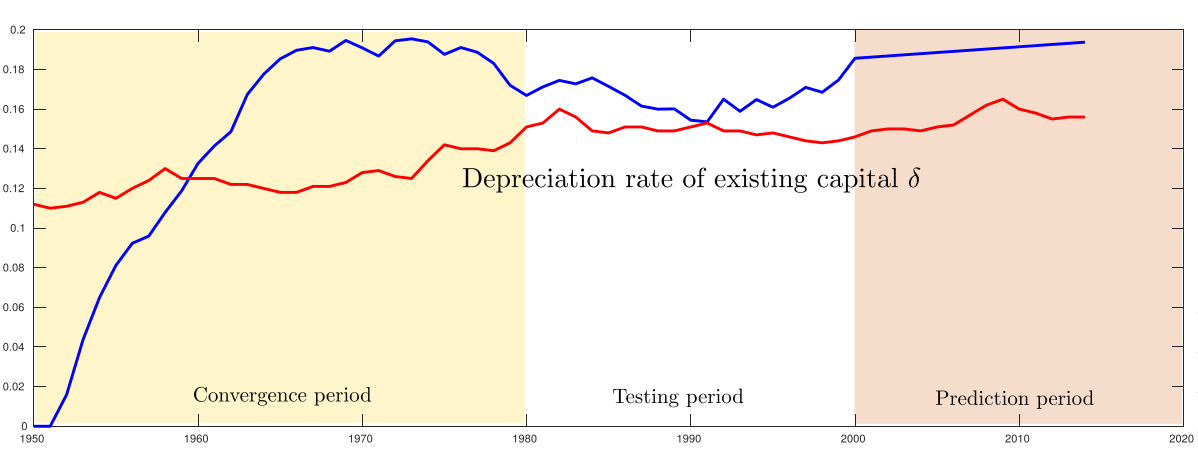
\includegraphics[width=6.2cm, height=5.2cm]{chart.png}

شکل 5:نرخ استهلاک
$\delta$
در مقاله‌ی مبنا

\end{center}





















\newtitle{۷. نتیجه‌گیری}


در این مقاله، در عین حال که مشکلاتی که برای مدل و داده‌ها وجود داشت، توانستیم به نتایج جالبی برای برخی از پارمترها دست یابیم. همانطور که در نمودار‌ها می‌بینیم، بعضی از پارامتر‌ها مثل 
$k$
و
$n$
حتی پس از اینکه دیگر به آن‌ها داده‌ای ندادیم همگرایی خوبی داشتند. اما انحرافات فاحشی نیز در برخی از تخمین‌ها به چشم می‌خورد. 

نتیجه‌ای که ما گرفتیم، نتایج مقاله‌ی 
\cite{main}
را نیز تایید می‌کرد، و هرچه از اندازه‌های بیشتری استفاده کردیم، تخمین‌هایمان به داده‌های واقعی نزدیک‌تر شدند. در قسمت بعد، در رابطه با ایده‌هایی که برای ادامه‌ی کار داشتیم توضیح می‌دهیم. همچنین در فرصت‌های آینده شروع به اعمال فیلترها و روش‌های گفته شده می‌کنیم و امیدواریم که نتایج گرفته شده قابل اطمینان‌تر باشند.





























\newtitle{۸. ادامه‌ی مسیر}


مقاله‌ی
\cite{main}
 ایده‌های جدیدی را مطرح کرده است. برای مثال، این اولین بار بوده است که از یک روش فیلترینگ غیرخطی برای تخمین مدل سولو-کاب-داگلاس استفاده شده است، و اولین بار بوده است که خاصیت‌های مشاهده‌پذیری این مدل غیرخطی بررسی شده‌اند. 

در این مقاله، برای تکنیک تخمین زدن از EKF استفاده کرده‌ایم. دلیل این انتخاب این است که EKF نقطه‌ی شروع مناسبی برای استفاده از تخمین‌هایی با روش فیلترینگ غیرخطی برای این مدل از مسائل است. در عین حال لازم است که دقت کنید که به این منظور می‌توان از روش‌های دیگر تخمین‌ با استفاده از فیلترینگ غیرخطی نیز استفاده کرد.

نتایج تئوری به دست آمده از آنالیز مشاهده‌پذیری نه تنها می‌توانند برای آزمایش قابل استفاده بودن EKF استفاده شوند بلکه می‌توانند برای سایر تکنیک‌های تخمین زدن بر مبنای فضا-حالت
\LTRfootnote{State-space}
نیز استفاده شوند. ار آنجایی که مشاهده‌پذیری یک خاصیت ذاتی سیستم است، در صورت استفاده از سایر روش‌ها نیز تمامی روابط و مراحل بالا برقرار هستند، و می‌توانیم از آن‌ها استفاده کنیم.

با توجه به موارد گفته شده، گام بعدی پس از بهینه‌سازی کد استفاده شده (به خصوص روی داده‌های ایران) این است که فیلتر‌های دیگری مثل
PF
و
UKF
استفاده کنیم. انتظار داریم که این فیلترها نتایج بهتری نسبت به
EKF
به ما بدهند زیرا همانطوری که در مقاله اشاره کردیم، 
EKF
با تمام جزئیاتش از ساده‌ترین و ابتدایی ترین روش‌های فیلتر کردن است و به طبع استفاده از روش‌های پیچیده‌تری مثل UKF ما را به نتیجه‌های بهتری می‌رسانند.

\end{multicols}





















\newtitle{۹. منابع}

\newhline
\begin{LTR}
\begin{thebibliography}{99}

\bibitem{s1}
Rger Labbe. Kalman and Bayesian Filter in Python. \url{https://github.com/rlabbe/Kalman-and-Bayesian-Filters-in-Python.git}

\bibitem{s2}
  Statistical Centre of Iran. \url{http://Amar.org.ir}

\bibitem{s3}
World Bank Data. \url{http://data.worldbank.ir}

\bibitem{main}
Estimation of the Solow-Cobb-Douglas economic growth model with a
Kalman filter: An observability-based approach. \url{https://europepmc.org/backend/ptpmcrender.fcgi?accid=PMC6595187&blobtype=pdf}
\end{thebibliography}
\end{LTR}
\end{document}
